%!TEX root=report.tex
\subsection{GMM clustering results}
First a matrix $X$ with dimensions 64800x341 ( positions on the rows, observations on columns) was constructed. Then the dimensionality reduction was needed. From the previous KMeans results, a ballpark estimate was made: It was assumed that anywhere from five to fifteen percent of the variance in the data was due to noise. Thus aiming for PCs explaining around 90 percent of the variance, in the the ten most principal components was chosen; in total they accounted for $91.6\%$ of the variance in the original $X$ space.
\\
As in the KMeans case the number of clusters chosen was 8. The algorithm converged on the following clusters (centroids are shown on the next page).
\begin{figure}[H]
	\center
	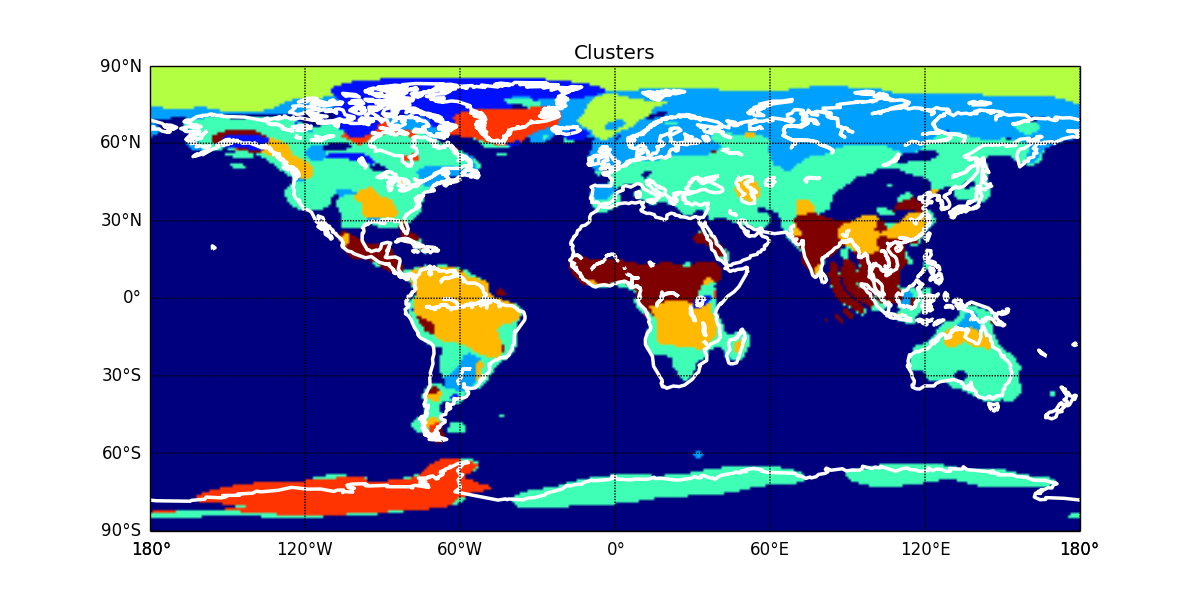
\includegraphics[width=\textwidth]{figures/gmm_world_8_clusters.png}
	\caption{GMM clusters}
\end{figure}
\begin{figure}[H]
	\center
	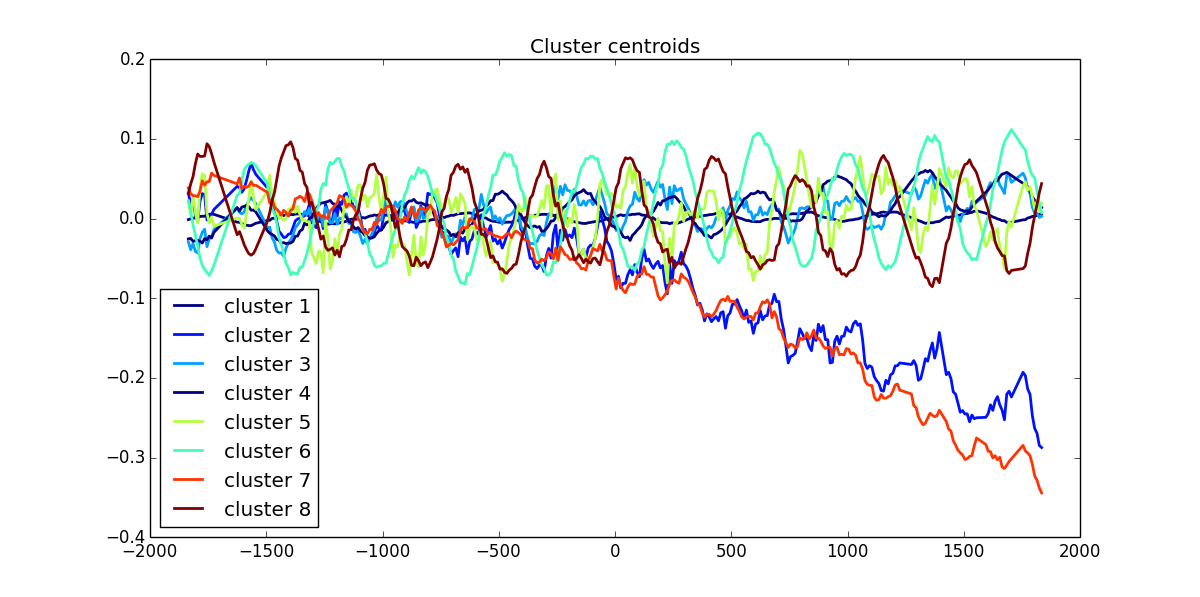
\includegraphics[width=\textwidth]{figures/gmm_8_clusters.png}
	\caption{GMM centroids}
\end{figure}
\todo{comment when final number of clusters is decided.}
The 1.96 times the square root of diagonal of the covariance matrices for each cluster is shown in a table in appendix \ref{GMM-covariance-appendix}.